\section*{Introduction}
    \paragraph{}
    Dans ce chapitre, nous présentons les résultats des simulations faites pour tester le fonctionnement de notre solution. Dans un premier temps,
    nous allons présenter l’application, une attaque pour tester la s\'ecurit\'e de notre r\'eseau et nous aborderons ensuite une discussion.


    \section{Présentation des résultats des tests}
      \paragraph{}
	  \begin{figure}[H]
	      \begin{center}
		  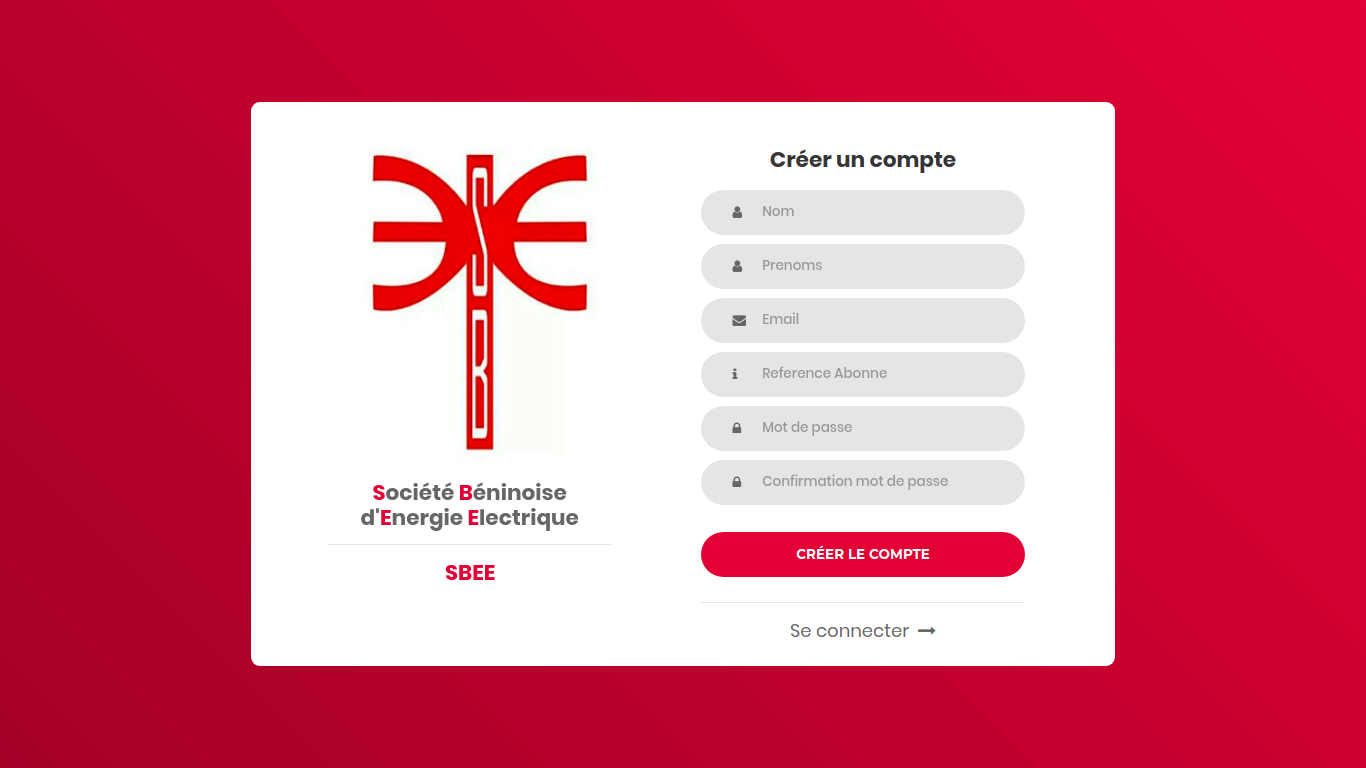
\includegraphics[scale=0.35]{images/register.png}
	      \end{center}
	      \caption{Page d'inscription de l'application}
	      \label{Accueil}
	  \end{figure}
	  La figure 3.1 présente la page d'ouverture de compte de notre application. L'utilisateur entre son nom, pr\'enom(s), adresse email, la r\'ef\'erence abonn\'ee et le mot de passe. Un mail d'activation lui est envoy\'e et il est redirig\'e vers la page de connexion.
	      
	  \begin{figure}[H]
	      \begin{center}
		  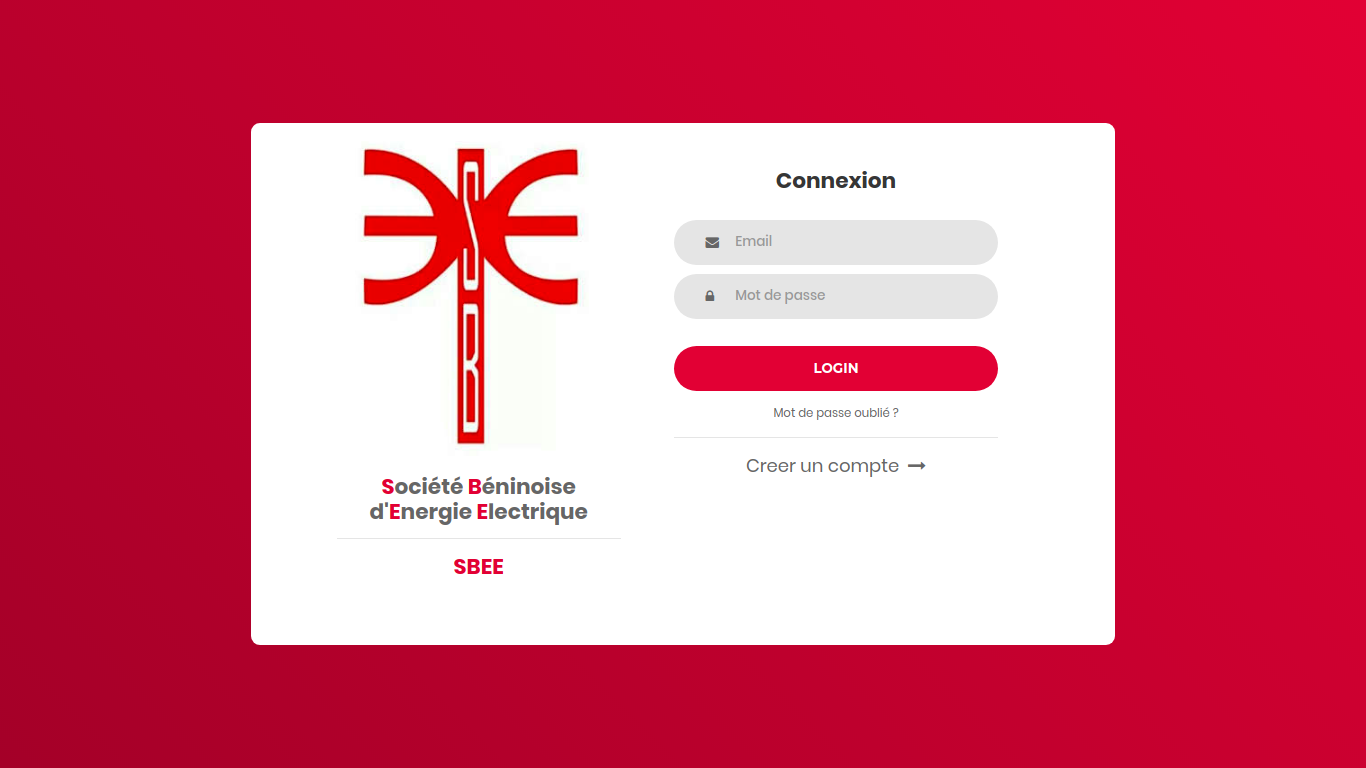
\includegraphics[scale=0.35]{images/login.png}
	      \end{center}
	      \caption{Page de connexion}
	      \label{Page de la whitelist IP}
	  \end{figure}
	  L'utilisateur entre son email et son mot de passe pour se connecter \`a l'application.
      
      \subsection{Interfaces Abonn\'e}
	  \begin{figure}[H]
	      \begin{center}
		  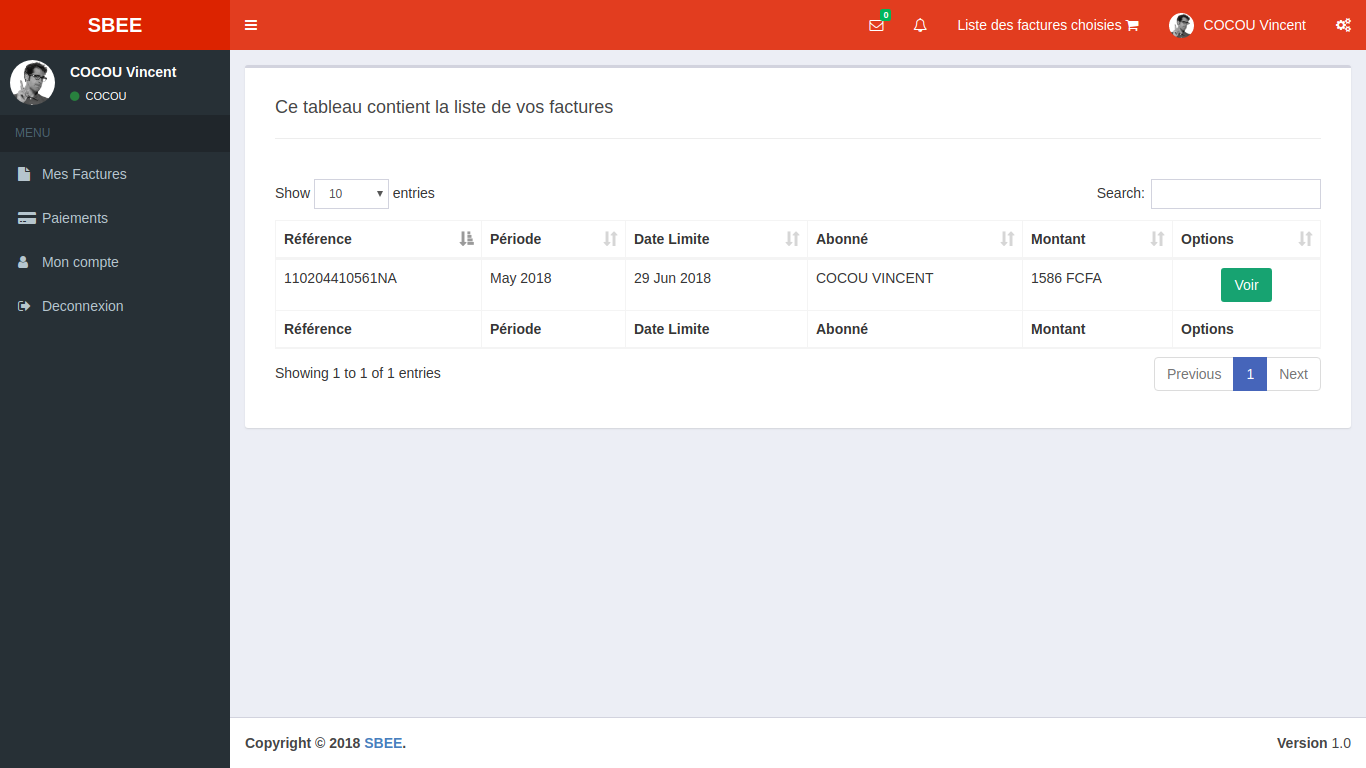
\includegraphics[scale=0.35]{images/listfactures.png}
	      \end{center}
	      \caption{Liste des factures de l'abonn\'e}
	      \label{Page de la whitelist Port}
	  \end{figure}
	  Tous les utilisateurs ont acc\`es \`a la liste de leurs factures. Ils peuvent cliquer sur le bouton \textbf{Voir} pour voir la facture sous le format habituel qu'ils connaissent (le format d'impression et de distribution), ou juste afficher les informations sous forme de liste.
			      
	  \begin{figure}[H]
	      \begin{center}
		  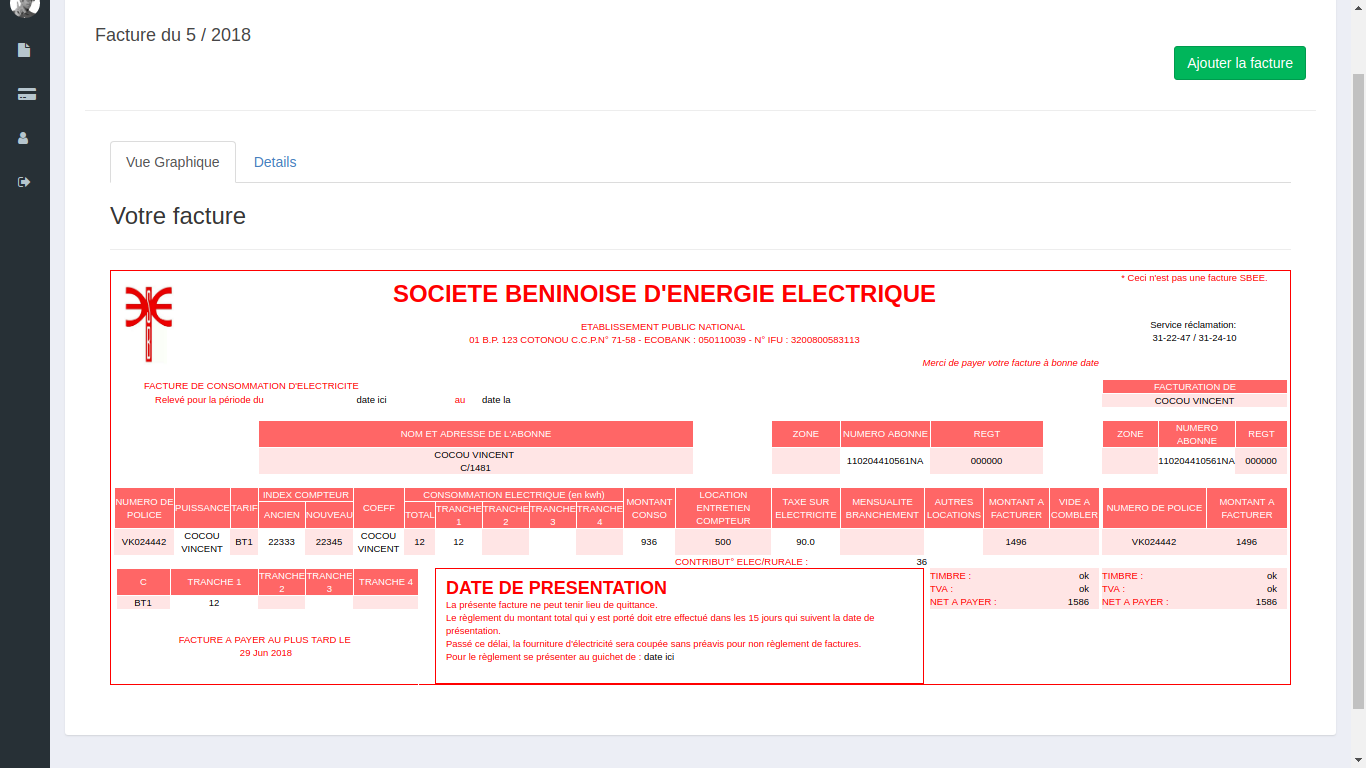
\includegraphics[scale=0.35]{images/graphic.png}
	      \end{center}
	      \caption{Vue d'une facture (Format d'impression)}
	      \label{Page de la whitelist Port}
	  \end{figure}
	  Il s'agit d'une repr\'esentation de la facture physique que nous connaissons tous.
						      
	  \begin{figure}[H]
	      \begin{center}
		  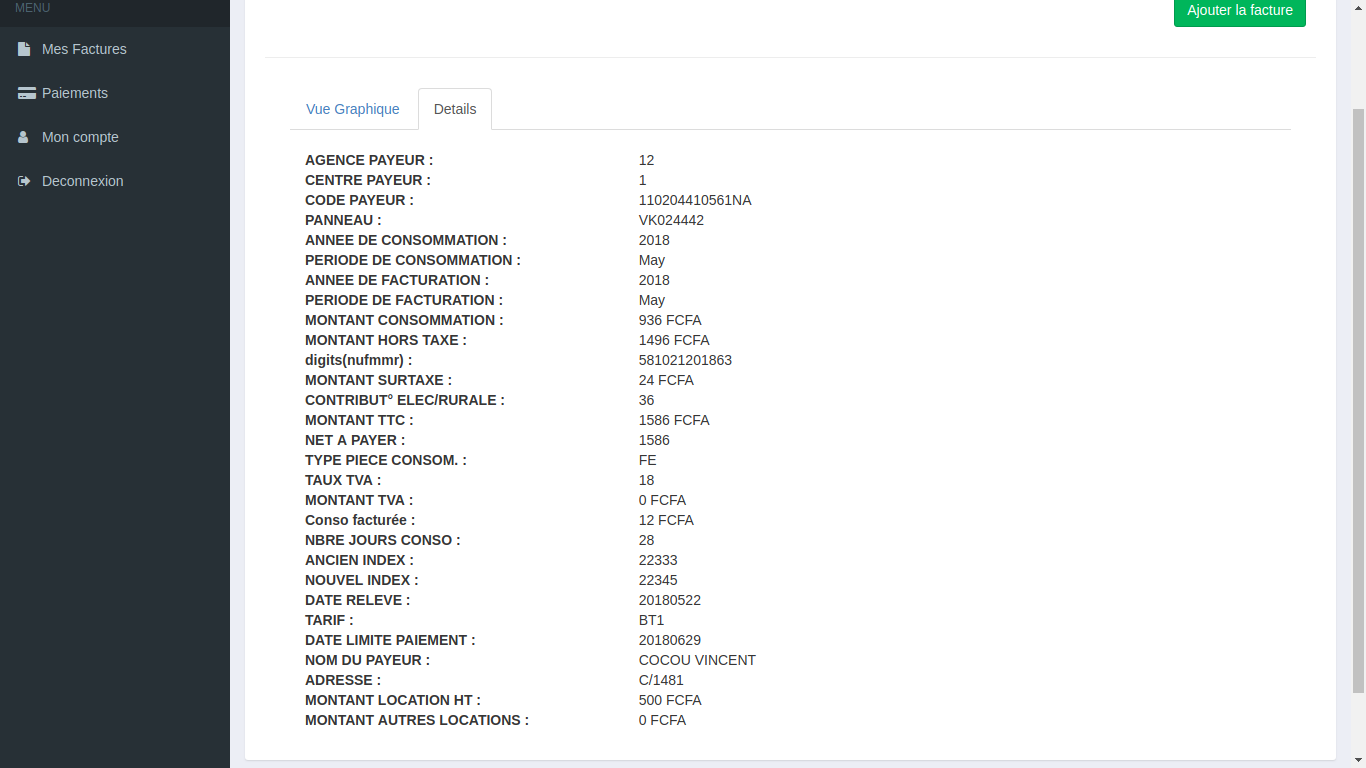
\includegraphics[scale=0.35]{images/details.png}
	      \end{center}
	      \caption{Vue d'une facture (Liste d'informations)}
	      \label{Page de la whitelist Port}
	  \end{figure}
	  Ce format permet d'avoir les informations d'une fa\c{c}on plus lisible et plus claire.
			      
	  \begin{figure}[H]
	      \begin{center}
		  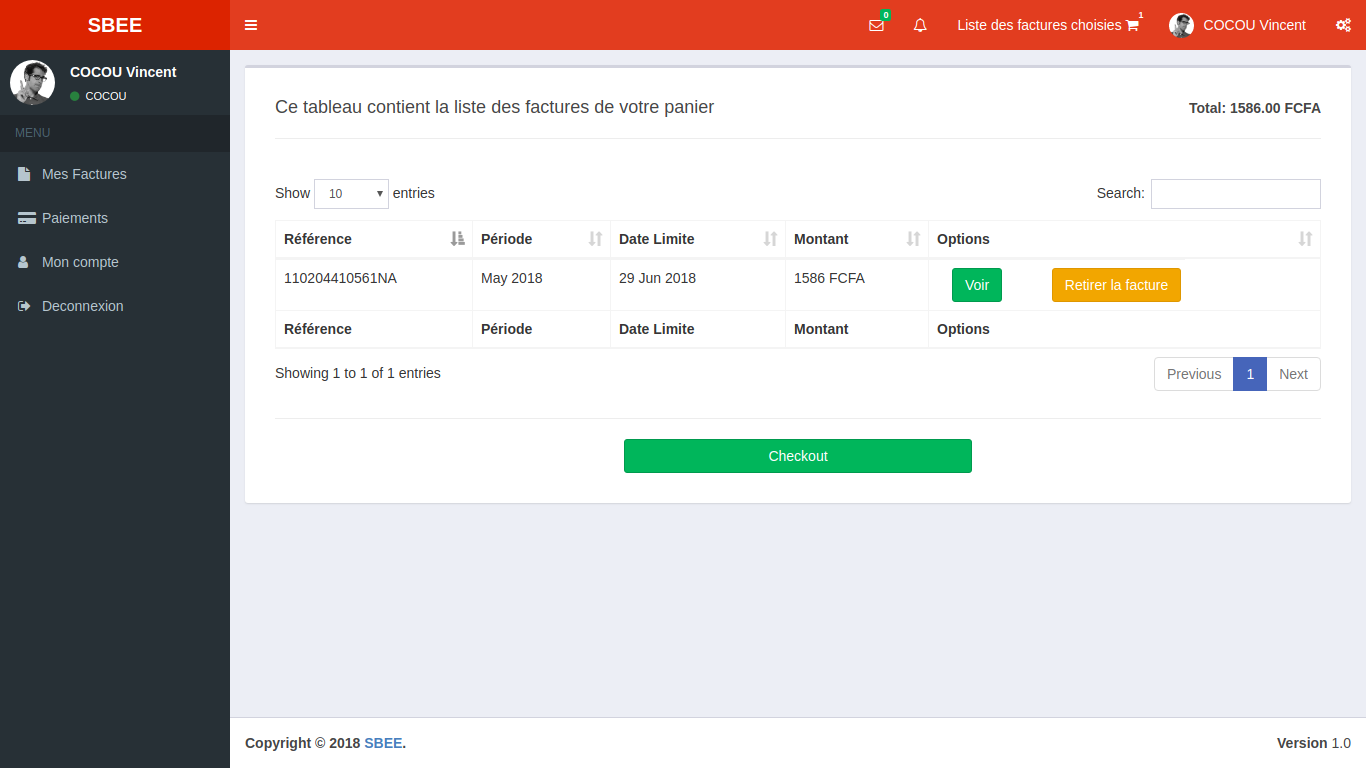
\includegraphics[scale=0.35]{images/choix.png}
	      \end{center}
	      \caption{Liste des factures choisies}
	      \label{Page de la whitelist Port}
	  \end{figure}
	  Afin de permettre de solder plusieurs factures en une fois, l'utilisateur choisit toutes les factures qu'il d\'esire r\'egler et ensuite il proc\`ede au checkout\footnote{Expression anglaise: régler la note, proc\'eder au paiement}.
			      
	  \begin{figure}[H]
	      \begin{center}
		  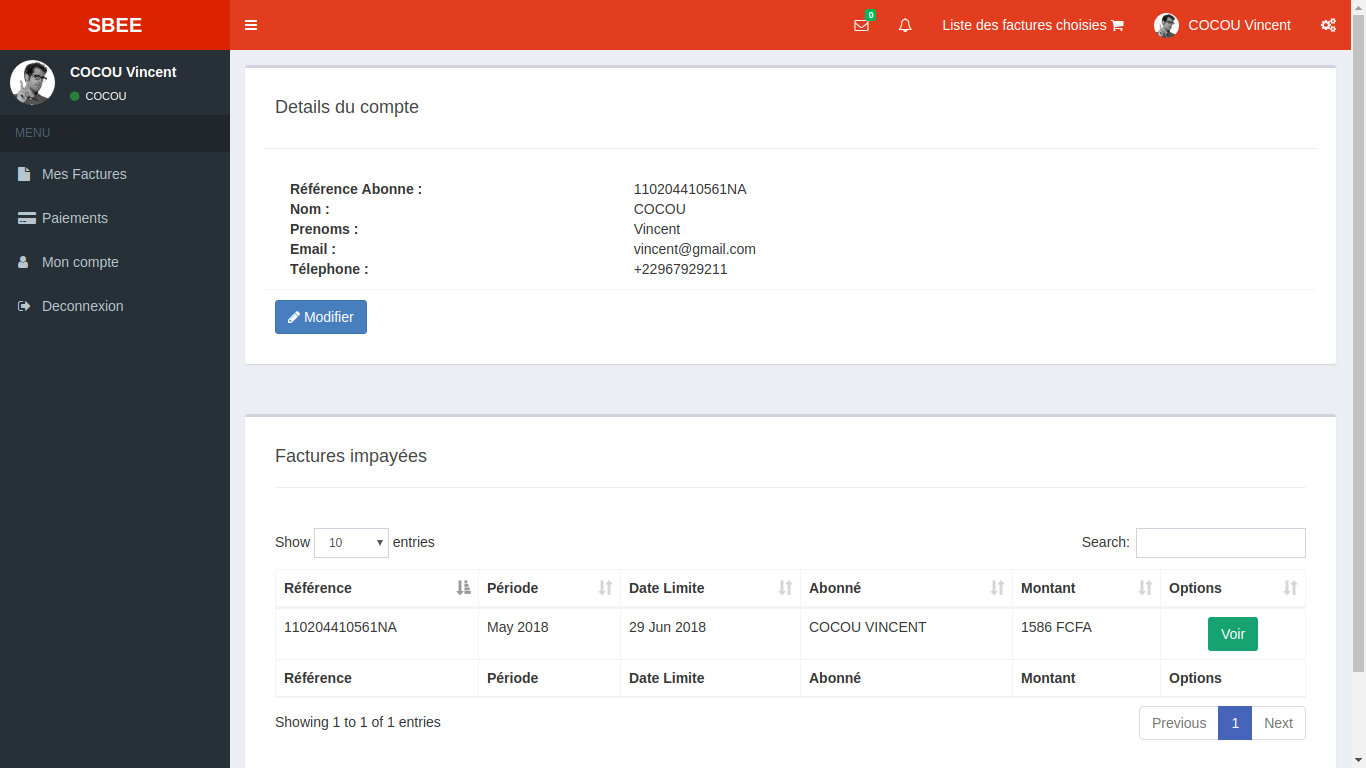
\includegraphics[scale=0.35]{images/detailcompte.png}
	      \end{center}
	      \caption{Le compte d'un utilisateur}
	      \label{Page de la whitelist Port}
	  \end{figure}
	  L'utilisateur a acc\`es aux informations de son compte. Et il peut actuellement modifier son nom, pr\'enom et num\'ero de t\'elephone.
		
      \subsection{Interfaces Administrateurs}
	 Les Administrateurs ont acc\`es \`a bien plus de fonctionnalit\'es que les abonn\'es simples:
	  \begin{itemize}
	    \item La liste des utilisateurs de la plateforme (abonn\'es simples et administrateurs)
	       \begin{figure}[H]
		  \begin{center}
		      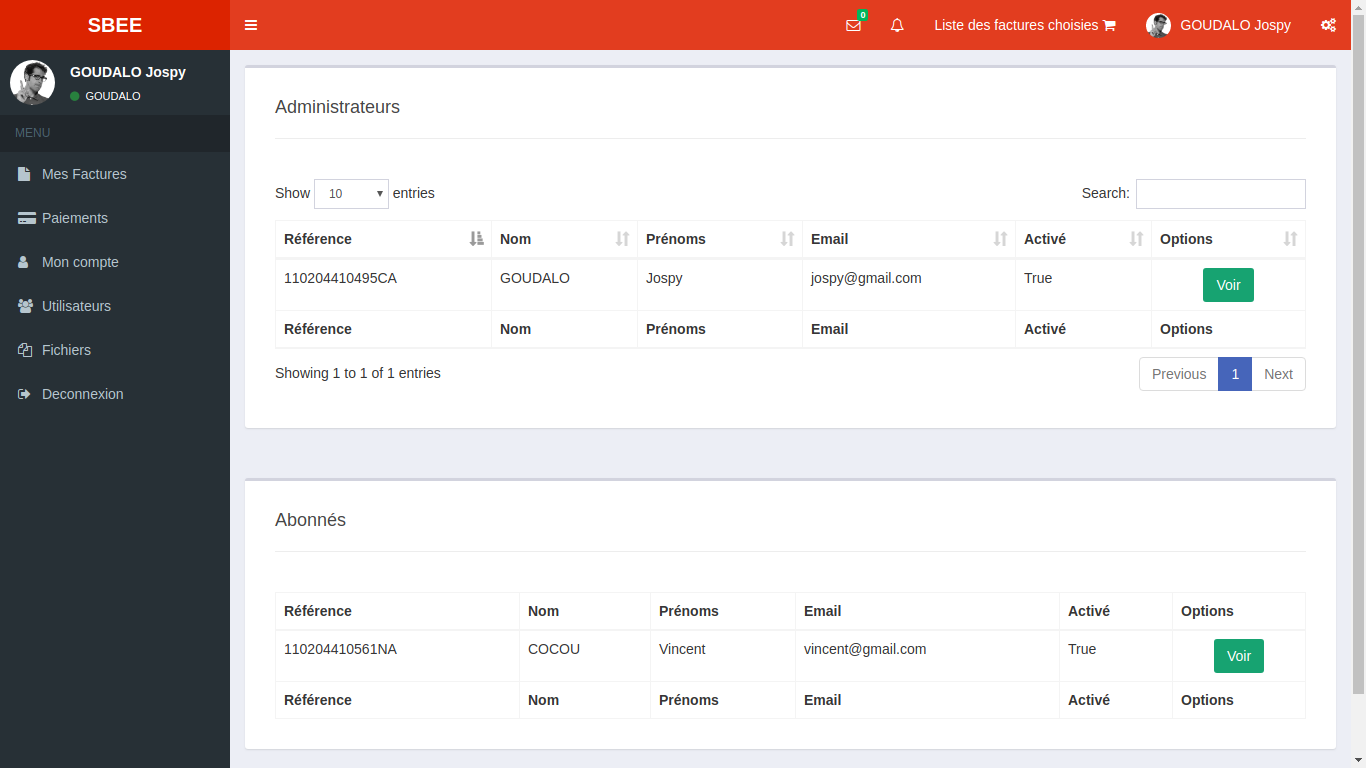
\includegraphics[scale=0.35]{images/gcv.png}
		  \end{center}
		  \caption{Utilisateurs de la plateforme}
		  \label{Page de la whitelist Port}
	      \end{figure}
	    
	    \item Les fichiers: la liste de tous les fichiers factures charg\'es dans la base de données ainsi que les r\`eglements,
	      \begin{figure}[H]
		  \begin{center}
		      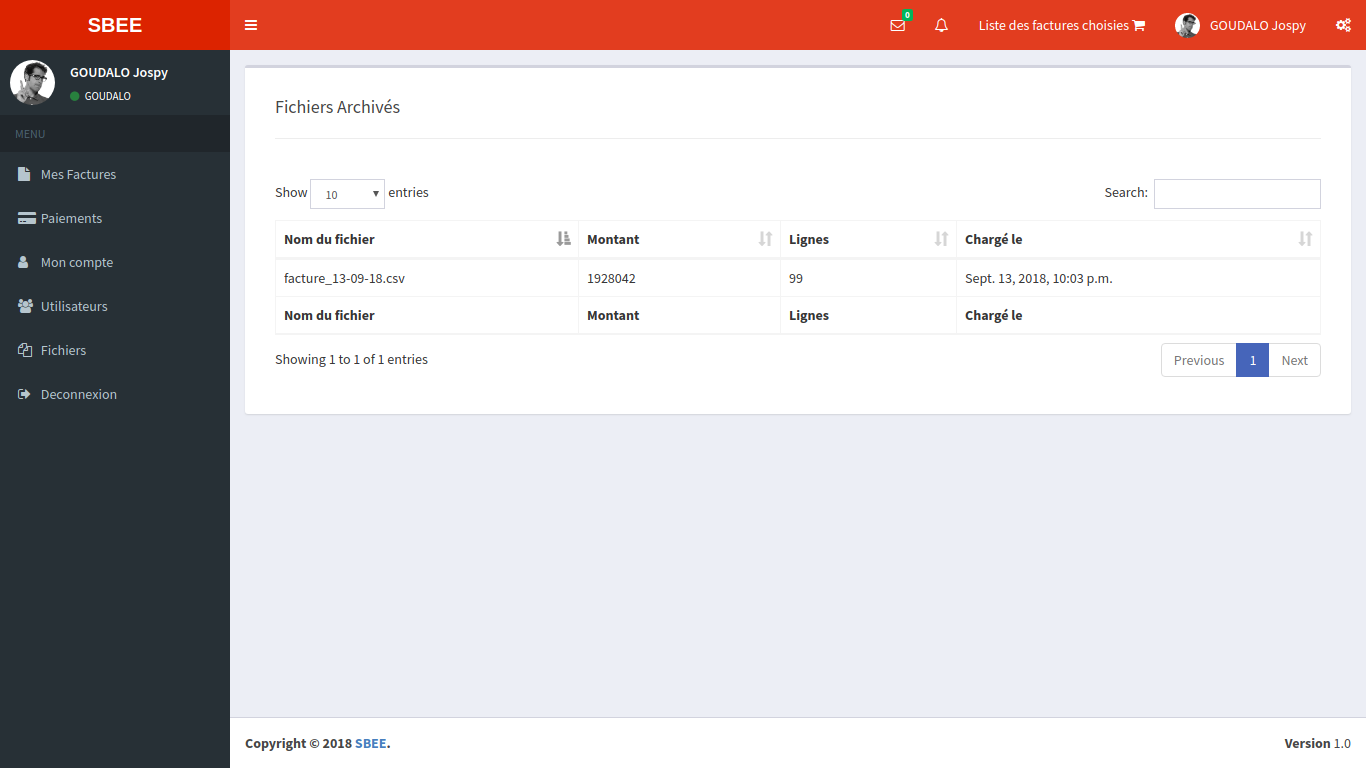
\includegraphics[scale=0.35]{images/files.png}
		  \end{center}
		  \caption{Fichiers import\'es}
		  \label{Page de la whitelist Port}
	      \end{figure}
	      
	  \end{itemize}

	      
    \section{Discussion}
	  \paragraph{}
	      Notre projet est né de plusieurs constats dont entre autre les pertes de temps dans les guichets de la SBEE, et les multiplications croissantes des attaques et intrusions informatiques. Des travaux n'ont pas encore \'et\'e faits \`a l'interne dans les locaux de la SBEE pour palier \`a ces probl\`emes observ\'es. Ceci repr\'esente donc un premier pas fait vers le paiement des factures num\'eriques.
	      
	  \paragraph{}
	      Ainsi, d'une part, notre solution est simple à utiliser et est utilisable depuis un navigateur web. Elle est accessible via internet et ne requiert aucun équipement ou installation spécifique chez l'utilisateur. Elle permet aux utilisateurs de consulter leurs factures et ainsi donc de suivre leur consommation plus facilement. Cependant la soci\'et\'e choisira elle-m\^eme via un appel d'offre ses prestataires pour les diff\'erentes solutions de paiement. Nous avons eu \`a faire quelques recommandations dont: \textbf{Mobile Money de MTN} ainsi que le service mondialement reconnu \textbf{PayPal}.
	      
	  \paragraph{}
	      Aussi existe-t-il des risques de double paiements lors des factures. Etant donn\'e que Gd'Or fonctionne en mode non connect\'e et que les factures ne sont valid\'ees qu`apr\`es 00h, un utilisateur qui va en agence pourrait payer une facture qui a d\'ej\`a \'et\'e pay\'ee en ligne. Cependant ces cas seront rembours\'es par les acteurs des diff\'erentes solutions de paiement car Gd'Or d\'etecte automatiquement les doublures lors de l'apurement des comptes et renvoie des fichiers contenant les erreurs aux entit\'es correspondantes. Celle derni\`ere proc\'edera \`a un remboursement des fonds aux utilisateurs concern\'es.

	  \paragraph{}
	      D'autre part, l'architecture et les outils propos\'es nous permettent d'assurer un minimum de s\'ecurit\'e pour notre application et dans notre r\'eseau. Notre strat\'egie se base essentiellement sur la maitrise du flux de donn\'ees et de la connaissance effective de chaque entit\'e du r\'eseau. Et ceci est un prérequis pour assurer la sécurité : \textbf{On ne protège bien que ce que l’on connaît}. Cependant cette architecture ne nous met pas à l’abri de toutes les attaques, mais nous prot\`ege quand m\^eme contre beaucoup d'attaques courantes, ce qui n’est pas négligeable.

	      
    \section*{Conclusion}
	  \paragraph{}
		  Dans ce chapitre, nous avons exposé les résultats des tests de notre application et réalisé quelques critiques concernant ses performances et ses insuffisances. Ces insuffisances peuvent être perçues comme des perspectives afin d'améliorer le travail fait pour une utilisation plus efficiente.